\section{eo\-CMABreed$<$ Fit\-T $>$ Class Template Reference}
\label{classeo_c_m_a_breed}\index{eoCMABreed@{eoCMABreed}}
TODO, handle bounds.  


{\tt \#include $<$eo\-CMABreed.h$>$}

Inheritance diagram for eo\-CMABreed$<$ Fit\-T $>$::\begin{figure}[H]
\begin{center}
\leavevmode
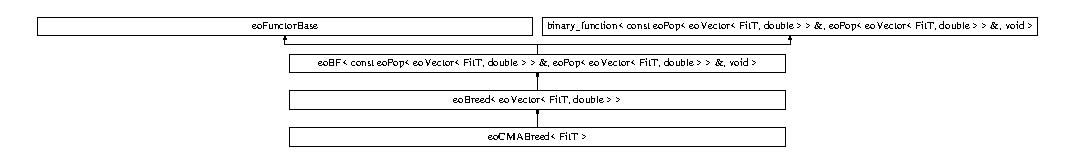
\includegraphics[height=1.73643cm]{classeo_c_m_a_breed}
\end{center}
\end{figure}
\subsection*{Public Member Functions}
\begin{CompactItemize}
\item 
{\bf eo\-CMABreed} (eo::CMAState \&state\_\-, unsigned lambda\_\-)\label{classeo_c_m_a_breed_a0}

\item 
void {\bf operator()} (const {\bf eo\-Pop}$<$ {\bf EOT} $>$ \&parents, {\bf eo\-Pop}$<$ {\bf EOT} $>$ \&offspring)\label{classeo_c_m_a_breed_a1}

\end{CompactItemize}
\subsection*{Private Types}
\begin{CompactItemize}
\item 
typedef {\bf eo\-Vector}$<$ {\bf Fit\-T}, double $>$ {\bf EOT}\label{classeo_c_m_a_breed_y0}

\end{CompactItemize}
\subsection*{Private Attributes}
\begin{CompactItemize}
\item 
eo::CMAState \& {\bf state}\label{classeo_c_m_a_breed_r0}

\item 
unsigned {\bf lambda}\label{classeo_c_m_a_breed_r1}

\end{CompactItemize}


\subsection{Detailed Description}
\subsubsection*{template$<$class Fit\-T$>$ class eo\-CMABreed$<$ Fit\-T $>$}

TODO, handle bounds. 



Definition at line 36 of file eo\-CMABreed.h.

The documentation for this class was generated from the following file:\begin{CompactItemize}
\item 
eo\-CMABreed.h\end{CompactItemize}
